\chapter{Specifica dei requisiti}
\section{Requisiti funzionali}
In questa sezione si vanno a specificare, secondo il rigoroso 
formalismo tabellare di A. Cockburn due degli use case ritenuti 
più significativi e centrali.
\subsection{Ricerca Immobili}
% Per tabelle che occupano più di una pagina:
%  longtblr al posto di tblr
\begin{longtblr}[
    caption = {Diagramma di Cockburn del caso d'uso \textit{Ricerca Immobili}.}
]{
    width = 10cm, %per fissare una larghezza
    column{1} = {3cm},
    column{2} = {0.8cm},
    column{3-4} = {3cm},
	vlines = {}, %per le cornici verticali
	hlines = {}, %per le cornici orizzontali
    % Merge delle righe/colonne:
    cell{1-7}{2} = {c = 3}{10cm, halign = l},
    cell{8}{1} = {r = 7}{valign = t},
    cell{15}{1} = {r = 3}{valign = t},
    cell{18}{1} = {r = 5}{valign = t},
    cell{23}{1} = {r = 2}{valign = t},
    cell{25}{1} = {r = 3}{valign = t},
    cell{28}{1} = {r = 3}{valign = t},
    cell{31}{1} = {r = 3}{valign = t},
    cell{34}{2} = {c = 3}{10cm, halign = l}
}
USE CASE & Ricerca Immobili & & \\
Goal in Context & Il Cliente vuole trovare annunci di immobili di suo interesse. & & \\
Preconditions & Nessuna precondizione. & & \\
Success End Condition & Il sistema tiene traccia della ricerca effettuata, salvandola tra le “Ricerche recenti”. & & \\
Fail End Condition & Il sistema tiene traccia della ricerca effettuata, salvandola tra le “Ricerche recenti”. & & \\
Primary Actor & Cliente & & \\
Trigger & Il Cliente clicca sulla barra di ricerca della schermata principale. & & \\
Main Scenario & Step & Cliente & Sistema   \\
 & 1 & Trigger & \\
 & 2 & & Mostra: 
 le eventuali ricerche recenti;
 la ricerca tramite punto sulla mappa. \\
 & 3 & Inserisce testo nella barra di ricerca.
 Seleziona il tipo di annuncio.
 Clicca su “Cerca”. & \\
 & 4 & & Mostra la schermata completa di ricerca. Mostrando i risultati. \\
 & 5 & Clicca su un risultato. & \\
 & 6 & & Mostra in sovrimpressione la schermata dettagliata dell’annuncio. Termina use case. \\
Extension A: 
click su una ricerca recente & Step & Cliente & Sistema \\
 & 3.a & Clicca su una ricerca recente. & \\
 & 4.a & & Torna allo step 4 del main scenario. \\
Extension B: 
ricerca tramite punto sulla mappa. & Step & Cliente & Sistema \\
 & 3.b & Clicca su “Ricerca tramite punto sulla mappa”. & \\
 & 4.b & & Mostra la schermata di ricerca tramite punto sulla mappa. \\
 & 5.b & Seleziona un punto sulla mappa, specificando un raggio di ricerca e clicca conferma. & \\
 & 6.b & & Torna allo step 4 del main scenario. \\

\pagebreak
Extension C:
la ricerca non ha prodotto risultati. & Step & Cliente & Sistema \\
 & 4.c & & Mostra la schermata “Non sono stati trovati risultati”. Torna allo step 2 del main scenario. \\
Extension D: nessun testo inserito.
 & Step & Cliente & Sistema \\
 & 3.d & non inserisce testo nella barra di ricerca e clicca su “Cerca”. & \\
 & 4.d & & Mostra messaggio “Inserisci una zona o un indirizzo”. Torna allo step 2 del main scenario. \\
Extension E: applica filtri. & Step & Cliente & Sistema \\
 & 5.e & Modifica dei filtri di ricerca. & \\
 & 6.e & & Torna allo step 4 del main scenario. \\
Extension F: annulla ultima operazione & Step & Cliente & Sistema \\
 & 5.b.f & Clicca sul pulsante annulla & \\
 & 6.b.f & & Torna allo step 2 del main scenario. \\
Open Issues & \begin{list}{+}{}
    \item Modellare o meno la barra di ricerca superiore?
    \item Modellare o meno il ritorno alla home con il click sul logo? E’ possibile scrivere una cosa del tipo Step:tutti per intendere che può avvenire in ogni step del Cliente?
\end{list} & & \\
\end{longtblr}
\begin{figure}[h]
    \centering
    \fbox{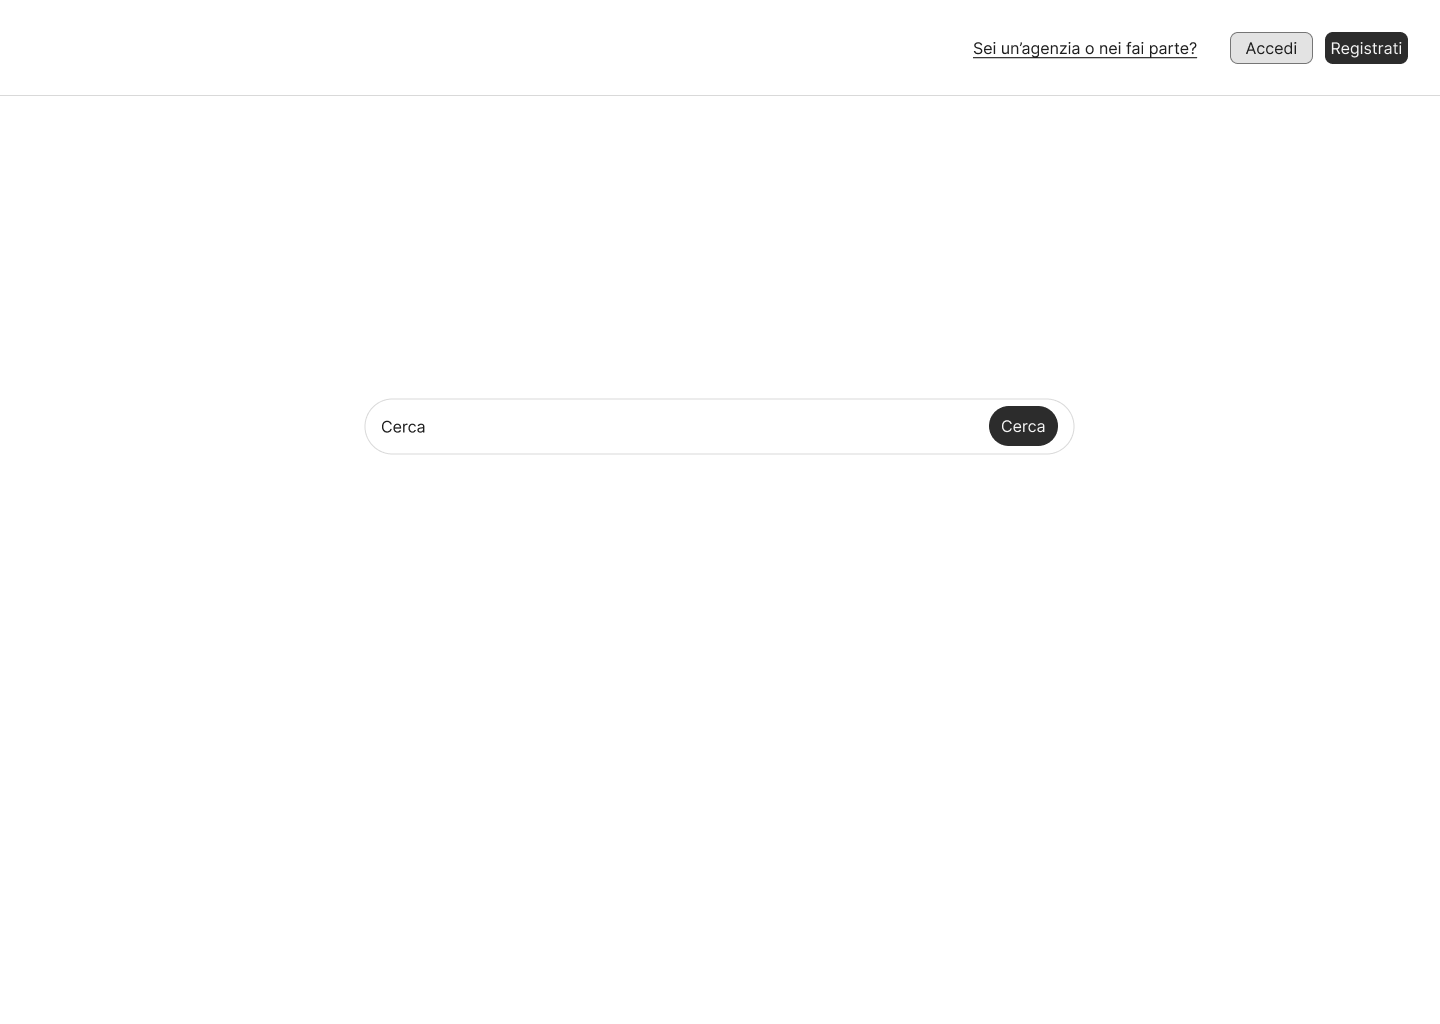
\includegraphics[width=\textwidth]{assets/mockups/ricerca-immobili/M-RI1.png}}
    \caption{M-RI1}
    \label{fig:M-RI1}
\end{figure}

\begin{figure}[h]
    \centering
    \fbox{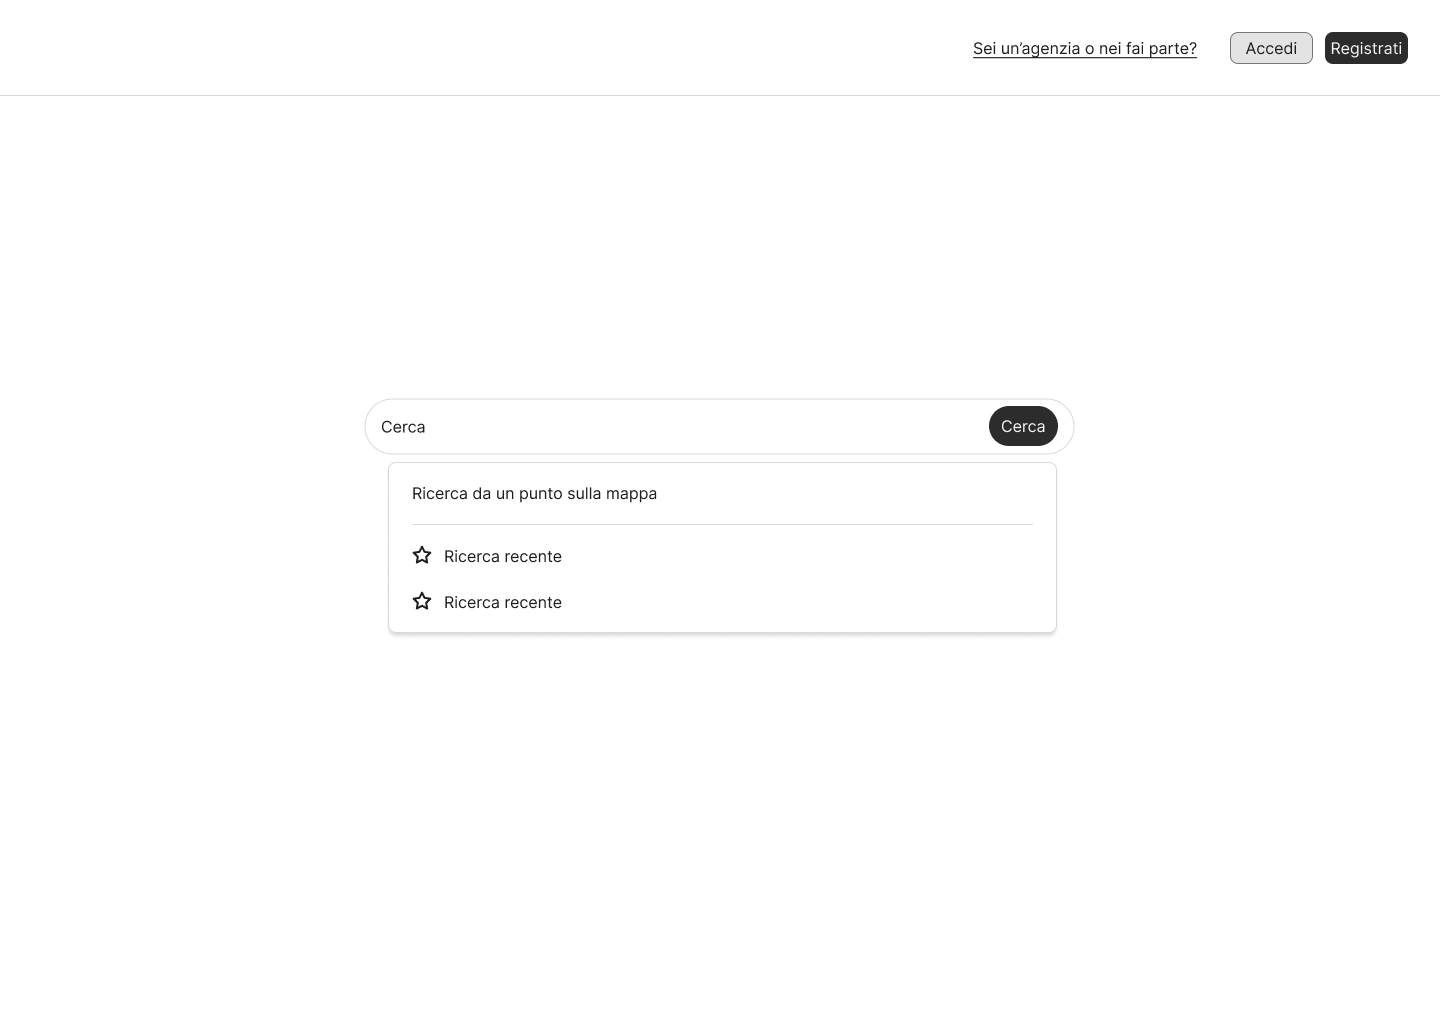
\includegraphics[width=\textwidth]{assets/mockups/ricerca-immobili/M-RI2.png}}
    \caption{M-RI2}
    \label{fig:M-RI2}
\end{figure}

\begin{figure}[h]
    \centering
    \fbox{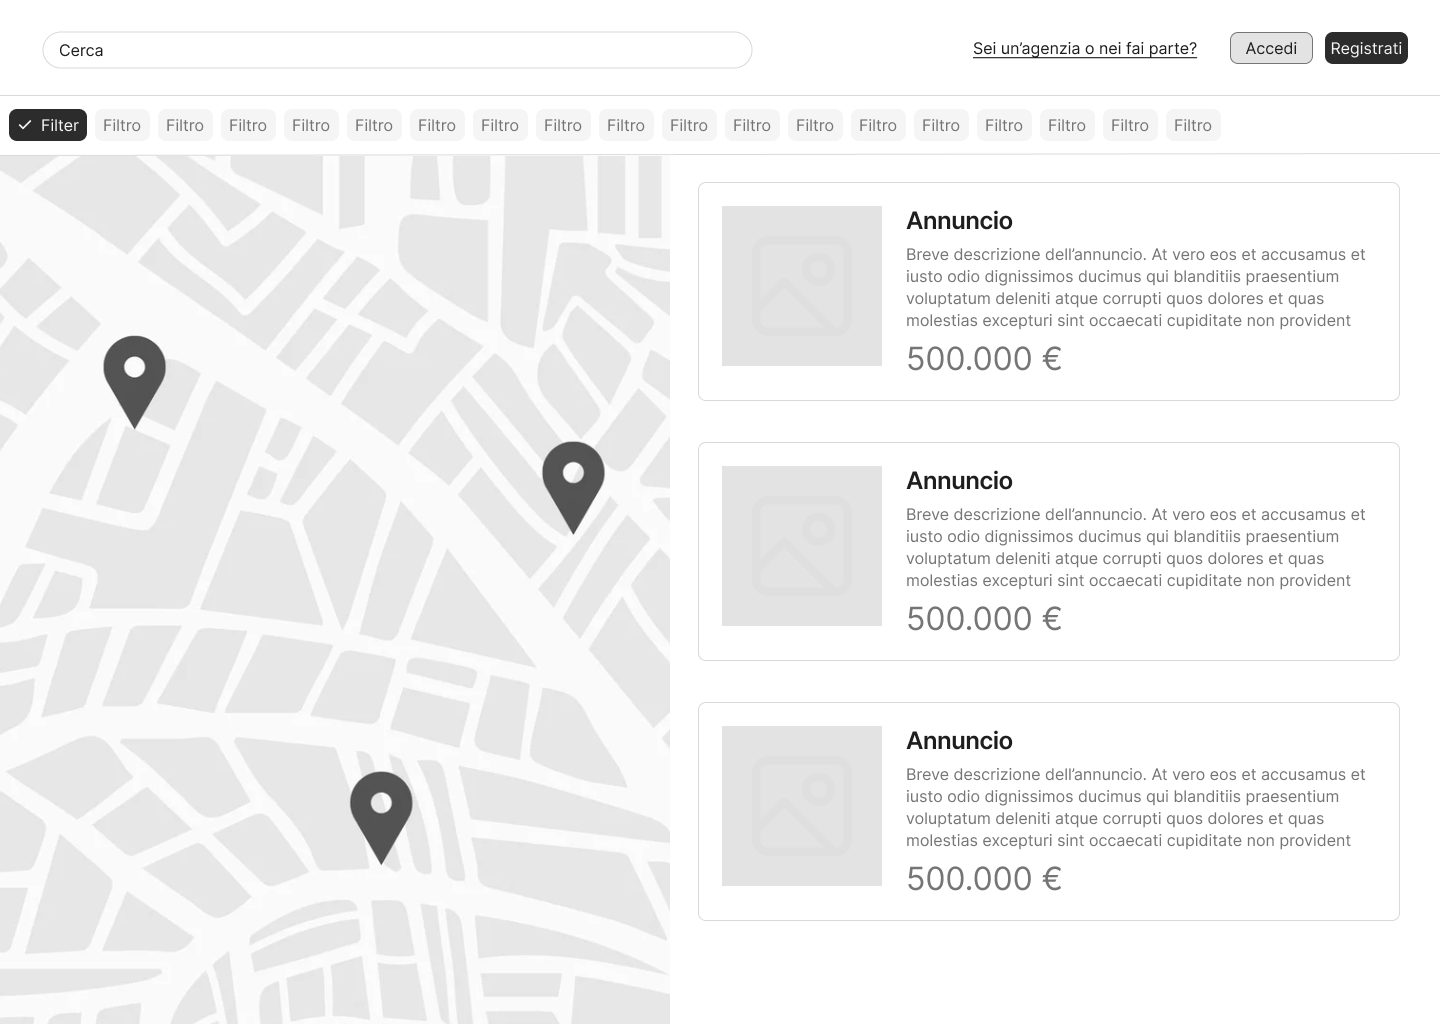
\includegraphics[width=\textwidth]{assets/mockups/ricerca-immobili/M-RI3.png}}
    \caption{M-RI3}
    \label{fig:M-RI3}
\end{figure}

\begin{figure}[h]
    \centering
    \fbox{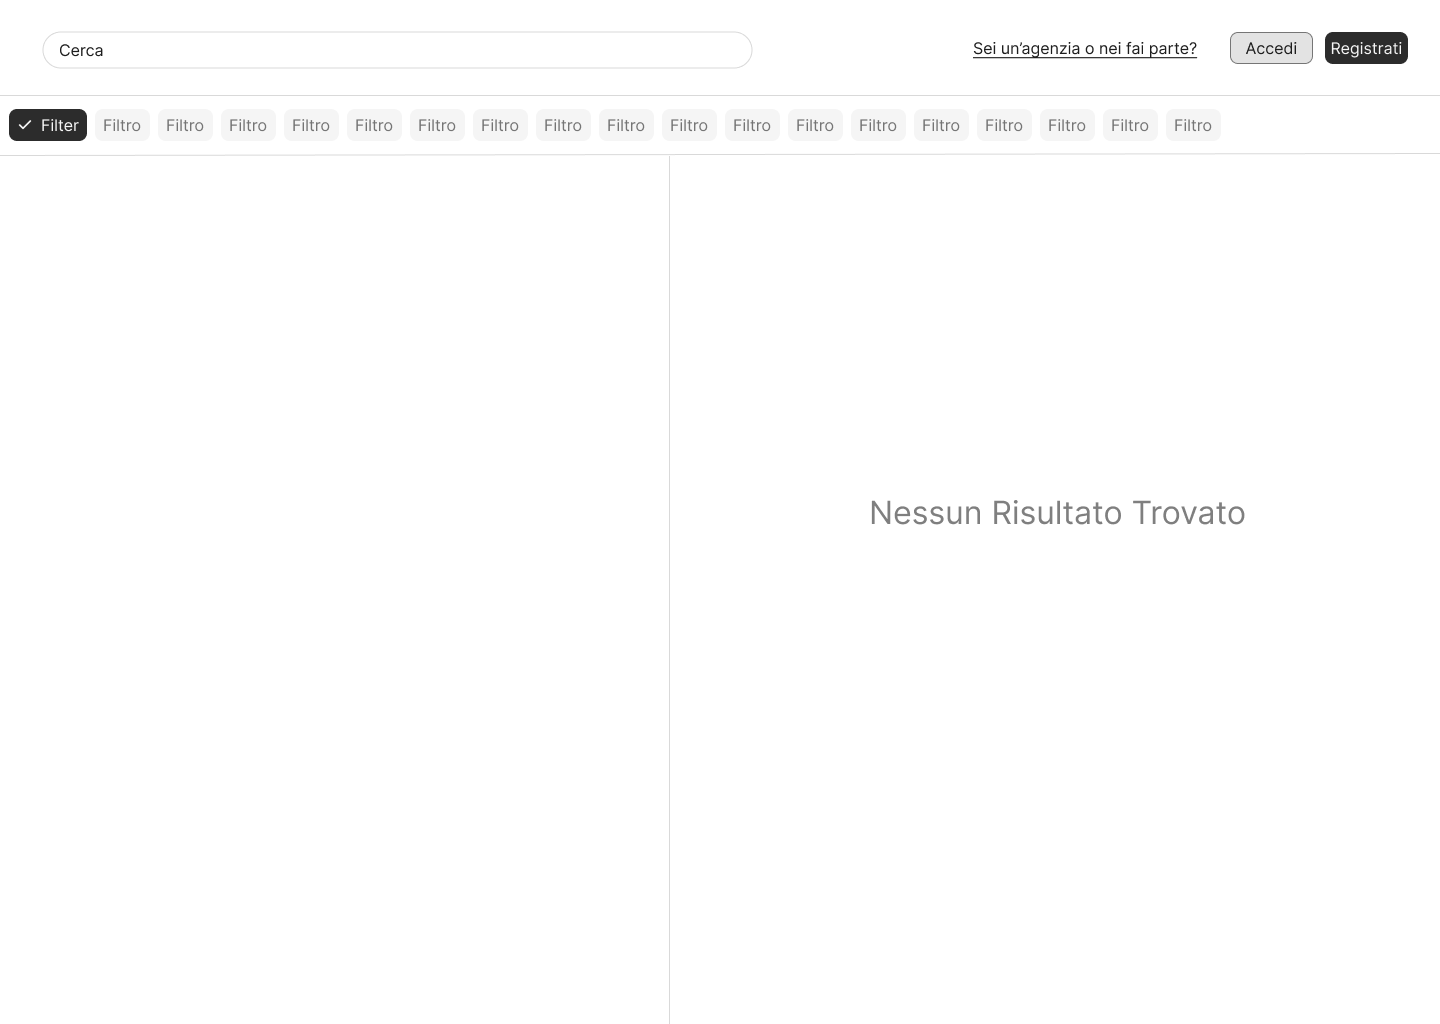
\includegraphics[width=\textwidth]{assets/mockups/ricerca-immobili/M-RI3bis.png}}
    \caption{M-RI3bis}
    \label{fig:M-RI3bis}
\end{figure}

\subsection{Fissa Appuntamento}
% Per tabelle che occupano più di una pagina:
%  longtblr al posto di tblr
\begin{longtblr}[
    caption = {Diagramma di Cockburn del caso d'uso \textit{Fissa Appuntamento}.}
]{
    column{1} = {3cm},
    column{2} = {0.8cm},
    column{3-5} = {3cm},
	vlines = {}, %per le cornici verticali
	hlines = {}, %per le cornici orizzontali
    % Merge delle righe/colonne:
    cell{1-7}{2} = {c = 4}{10cm, halign = l},
    cell{8}{1} = {r = 9}{valign = t},
    cell{17}{1} = {r = 3}{valign = t},
    cell{20}{1} = {r = 3}{valign = t},
    cell{23}{1} = {r = 3}{valign = t},
    cell{26}{2} = {c = 4}{10cm, halign = l}
}
USE CASE & Fissa appuntamento & & & \\
Goal in Context & Il Cliente vuole fissare un appuntamento con un Agente per la visione dell’immobile di interesse. & & & \\
Preconditions & Il Cliente deve essersi autenticato. & & & \\
Success End Condition & Il sistema tiene traccia della richiesta di appuntamento da parte del Cliente e la invia all’Agente. & & & \\
Fail End Condition & Il sistema non tiene traccia dell’attività non completata. & & & \\
Primary Actor & Cliente & & & \\
Trigger & Il Cliente preme il pulsante “Richiedi appuntamento” di \ref{fig:M-FA1}. & & & \\
Main Scenario   & Step & Cliente & Agente & System \\
 & 1 & Trigger action. & & \\
 & 2 & & & Mostra \ref{fig:M-FA2}. \\
 & 3 & Seleziona le sue preferenze. Clicca su Prosegui. & & \\
 & 4 & & & Mostra \ref{fig:M-FA3}. \\
 & 5 & Clicca su “Invia richiesta”. & & \\
 & 6 & & & Notifica al Cliente l'invio della richiesta. \\
 & 7 & & Accetta la richiesta. & \\
 & 8 & & & Notifica al Cliente la conferma dell’appuntamento e termina lo use case. \\
 
\pagebreak
Extension A & Step & Cliente & Agente & System \\
 & 3.a & Clicca su “Annulla”. & & \\
 & 4.a & & & Mostra \ref{fig:M-FA1} e termina use case.  \\
Extension B & Step & Cliente & Agente & System \\
 & 5.b & Clicca su “Annulla”. & & \\
 & 6.b & & & Torna allo step 2 del main scenario. \\
Extension C & Step & Cliente & Agente & System \\
 & 7.c & & Rifiuta la richiesta. & \\
 & 8.c & & & Invia al Cliente la notifica di rifiuto dell’appuntamento e termina lo use case. \\
Open Issues & & & & \\
\end{longtblr}
\begin{figure}[h]
    \centering
    \fbox{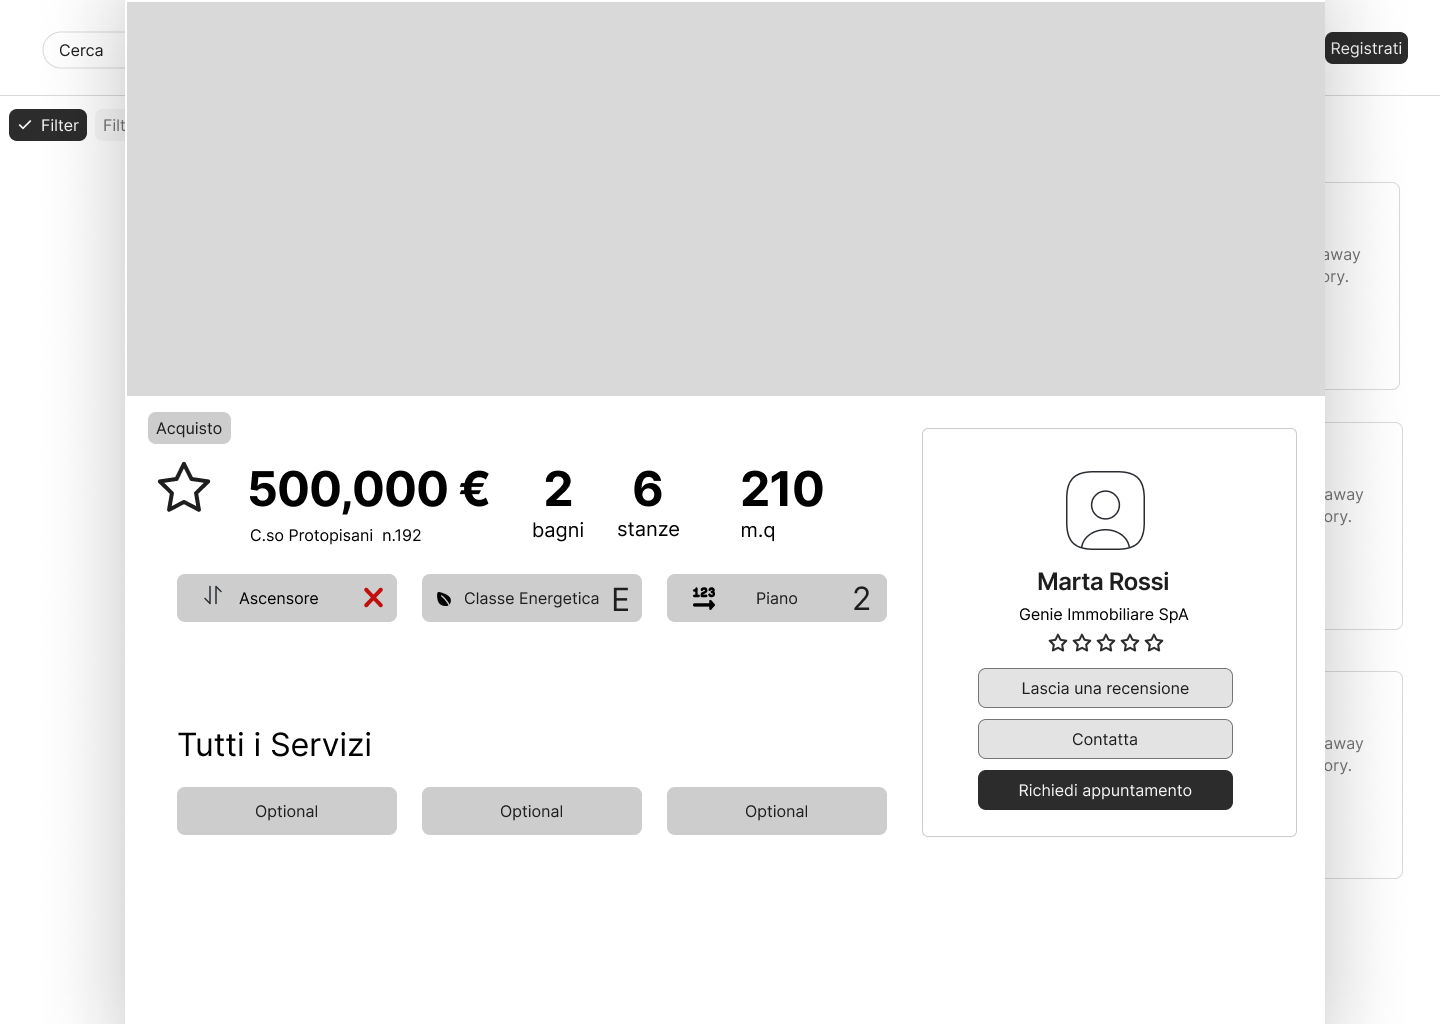
\includegraphics[width=\textwidth]{assets/mockups/fissa-appuntamento/M-FA1.png}}
    \caption{M-FA1}
    \label{fig:M-FA1}
\end{figure}
\begin{figure}[h]
    \centering
    \fbox{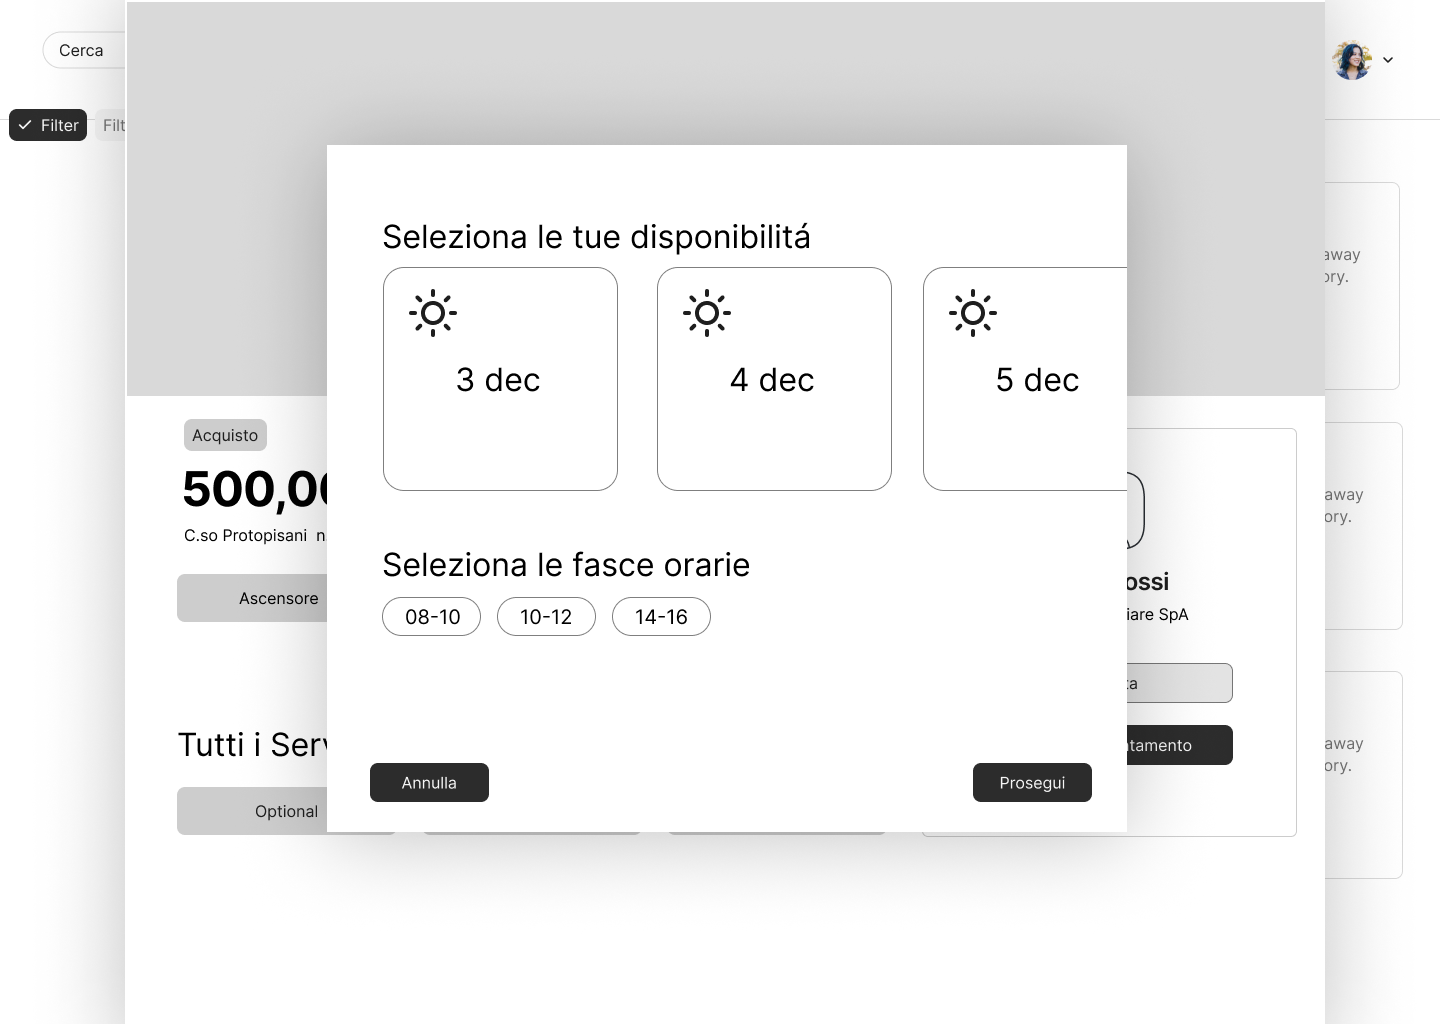
\includegraphics[width=\textwidth]{assets/mockups/fissa-appuntamento/M-FA2.png}}
    \caption{M-FA2}
    \label{fig:M-FA2}
\end{figure}
\begin{figure}[h]
    \centering
    \fbox{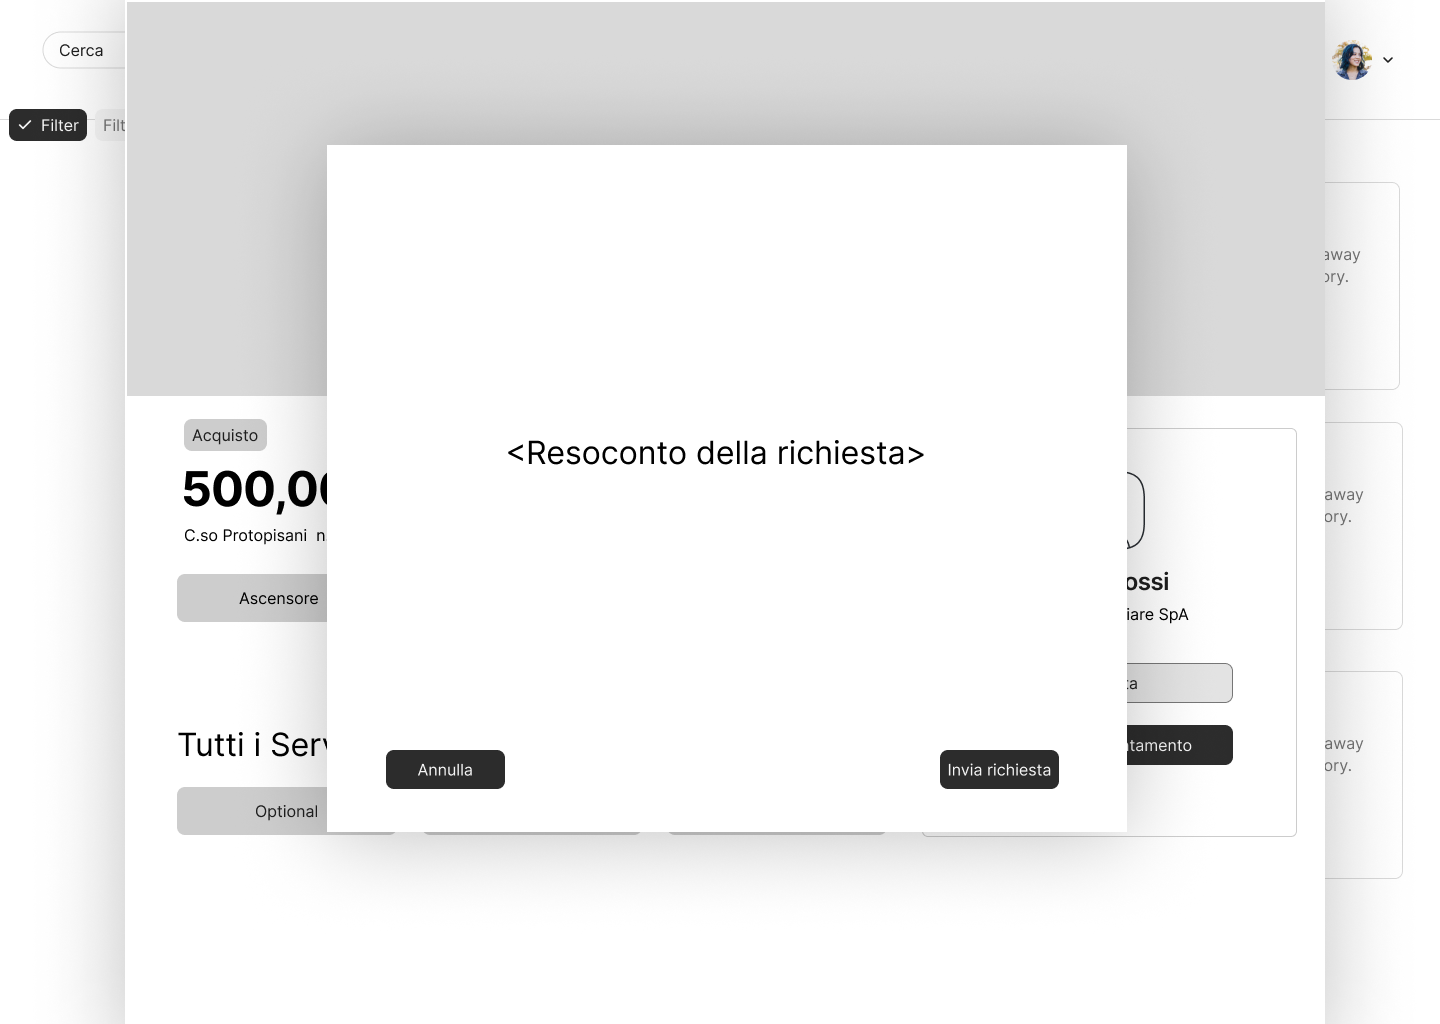
\includegraphics[width=\textwidth]{assets/mockups/fissa-appuntamento/M-FA3.png}}
    \caption{M-FA3}
    \label{fig:M-FA3}
\end{figure}

\subsection{Valuta Agente}
% Per tabelle che occupano più di una pagina:
%  longtblr al posto di tblr
\begin{longtblr}[
    caption = {Diagramma di Cockburn del caso d'uso Valuta Agente}
]{
    column{1} = {3cm},
    column{2} = {0.8cm},
    column{3-4} = {3cm},
	vlines = {}, %per le cornici verticali
	hlines = {}, %per le cornici orizzontali
    % Merge delle righe/colonne:
    cell{1-7}{2} = {c = 3}{10cm, halign = l},
    cell{8}{1} = {r = 5}{valign = t},
    cell{13}{1} = {r = 3}{valign = t},
    cell{16}{1} = {r = 3}{valign = t}
}
USE CASE & Valuta Agente & & \\
Goal in Context & Il Cliente vuole valutare la propria esperienza con un Agente & & \\
Preconditions & Il Cliente deve essere autenticato & & \\
Success End Condition & Il sistema tiene traccia della valutazione del Cliente & & \\
Fail End Condition & Il sistema non tiene traccia della valutazione del Cliente & & \\
Primary Actor & Cliente & & \\
Trigger & Il Cliente clicca sul pulsante "Aggiungi una recensione" della schermata \ref{fig:M-RI4} & & \\
Main Scenario & Step & Cliente & System   \\
 & 1 & Trigger & \\
 & 2 & & Mostra la schermata \ref{fig:M-VA1}\\
 & 3 & Inserisce una valutazione da una a cinque stelle e un commento. 
 Clicca poi sul pulsante "Invia Recensione". & \\
 & 4 & & Registra la recensione e termina caso d'uso. \\
 Extension A & Step & Cliente & System   \\
 & 3.a & Inserisce solo la valutazione, solo il commento, nessuna delle due. & \\
 & 4.a & & Mostra un messaggio di errore. Torna allo step 2 del main scenario. \\
Extension B & Step & Cliente & System   \\
 & 3.b & Clicca su un'altra parte dello schermo che non riguardi il popup per la recensione. & \\
 & 4.b & & Torna alla schermata precedente e termina use case. \\
\end{longtblr}
\begin{figure}[h]
    \centering
    \fbox{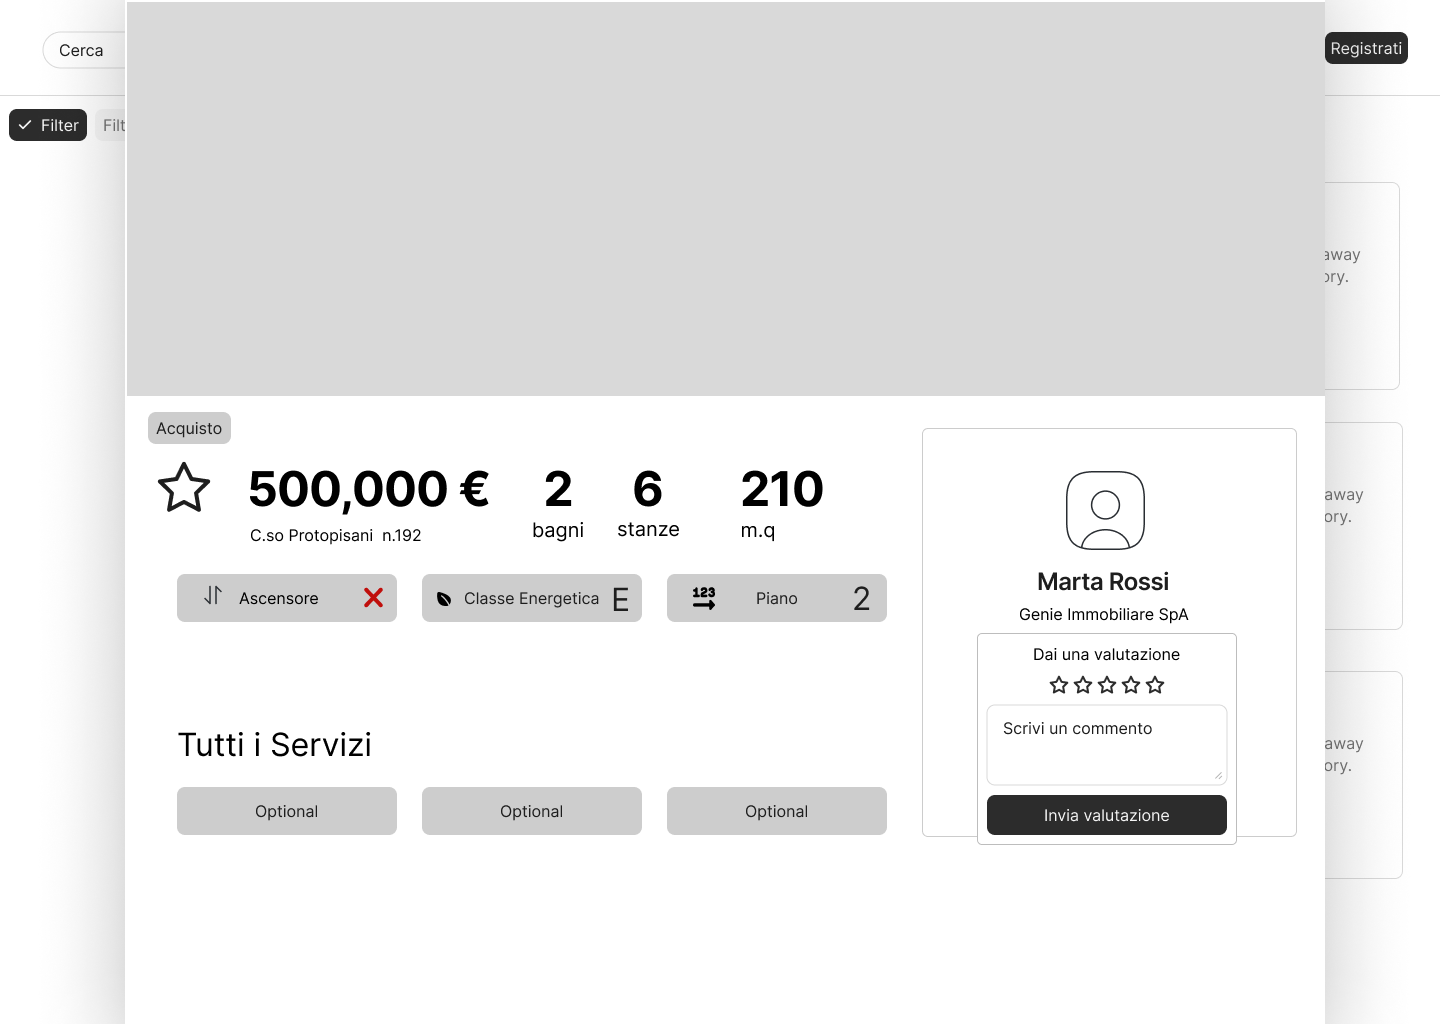
\includegraphics[width=\textwidth]{assets/mockups/valuta-agente/M-VA1.png}}
    \caption{M-VA1}
    \label{fig:M-VA1}
\end{figure}

\subsection{Salva Annuncio}
% Per tabelle che occupano più di una pagina:
%  longtblr al posto di tblr
\begin{tblr}[
    caption = {Diagramma di Cockburn del caso d'uso Salva Annuncio}
]{
    column{1} = {3cm},
    column{2} = {0.8cm},
    column{3-4} = {3cm},
	vlines = {}, %per le cornici verticali
	hlines = {}, %per le cornici orizzontali
    % Merge delle righe/colonne:
    cell{1-7}{2} = {c = 3}{10cm, halign = l},
    cell{8}{1} = {r = 3}{valign = t}
}
USE CASE & Salva Annuncio & & \\
Goal in Context & Il Cliente vuole salvare l'annuncio trovato tra i preferiti
in modo tale da accedervi piú velocemente in futuro & & \\
Preconditions & Il Cliente deve essersi autenticato & & \\
Success End Condition & Il sistema aggiunge l'annuncio tra gli annunci salvati
del Cliente & & \\
Fail End Condition & Il sistema non aggiunge l'annuncio tra gli annunci salvati
del Cliente & & \\
Primary Actor & Cliente & & \\
Trigger & Il cliente clicca sul pulsante a forma di stella presente sull'annuncio
d'interesse, nella schermata \ref{fig:M-RI4} & & \\
Main Scenario   & Step & Cliente & System   \\
 & 1 & Trigger & \\
 & 2 & & Tiene traccia dell'aggiunta ai preferiti e termina use case. \\
\end{tblr}

\section{Requisiti non funzionali}
Il sistema deve soddisfare le seguenti qualitá:
\begin{list}{$\cdot$}{}
    \item availability, una scarsa availability é causa di perdita di 
    credibilitá e di utenza.
    \item adaptability, un utente deve poter accedere al servizio da tutti 
    i dispositivi possibili.
    \item performance efficiency, un software di ricerca lento è un software 
    morto in partenza.
    \item usability, l'utente deve poter utilizzare appieno il software già 
    dal primo utilizzo.
    \item scalability, una qualitá imprescindibile per un sistema utilizzato 
    da, potenzialmente, milioni di persone contemporaneamente.
    \item maintainability, la qualitá, interna, fondamentale per il successo 
    di un software. Essa, se presente, garantisce al team produttivitá nel tempo.
\end{list}

Il sistema deve rispettare le prassi e le tecnologie allo stato dell'arte per 
garantire security, soprattutto dal lato della confidentiality, in ottica di 
rispetto della privacy e della sicurezza dei dati personali dell'utente.

\section{Requisiti di dominio}
Ciascun annuncio deve possere le seguenti caratteristiche obbligatorie:
\begin{list}{$\cdot$}{}
    \item Tipologia dell'immobile. Valore selezionabile da elenco predefinito 
    (appartamento, villa, terreno, ecc.)
    \item Superficie. Valore numerico espresso in metri quadri ($m^2$).
    \item Numero di locali (non previsto per alcune tipologie di immobile).
    \item Numero di bagni (non previsto per alcune tipologie di immobile).
    \item Piano (non previsto per alcune tipologie di immobile).
    \item Prezzo/canone.
    \item Classe energetica conforme alla classificazione APE (da A4 a G).
    \item Indirizzo e coordinate geografiche.
    \item Comune.
    \item Provincia.
    \item Contatto di un agente immobiliare.
    \item Titolo annuncio.
\end{list}

Le caratteristiche obbligatorie degli annunci potranno essere aggiornate in 
funzione di modifiche normative o esigenze di mercato. Il sistema deve essere 
progettato per adattarsi flessibilmente a tali variazioni con impatto minimo 
sull'architettura complessiva.